%% ===========================================================================
%% Cartify: An AI-Powered E-Commerce Recommendation System
%% IEEE conference format (IEEEtran, 2-column, US Letter).
%%
%% PAGE BUDGET: strict 6 pages max incl.\ references. 1 figure + 2 tables
%% only; body target ~4,200 words incl.\ captions. Tight spacing set in preamble.
%%
%% Compile: pdflatex -> bibtex -> pdflatex -> pdflatex
%% ===========================================================================
\documentclass[conference]{IEEEtran}

\usepackage[utf8]{inputenc}
\usepackage[T1]{fontenc}
\usepackage{amsmath,amssymb,amsfonts}
\usepackage{booktabs}
\usepackage{array}
\usepackage{graphicx}
\usepackage{textcomp}
\usepackage[hidelinks]{hyperref}
\usepackage{cite}
\setlength{\textfloatsep}{8pt plus 2pt minus 2pt}
\setlength{\floatsep}{8pt plus 2pt minus 2pt}
\setlength{\intextsep}{8pt plus 2pt minus 2pt}
\setlength{\abovecaptionskip}{4pt}
\setlength{\belowcaptionskip}{0pt}
\setlength{\abovedisplayskip}{4pt plus 1pt minus 2pt}
\setlength{\belowdisplayskip}{4pt plus 1pt minus 2pt}
\setlength{\tabcolsep}{3pt}

\usepackage{tikz}
\usetikzlibrary{arrows.meta,positioning,shapes.geometric}

\begin{document}

\title{Cartify: An AI-Powered E-Commerce Recommendation System}

\author{
\IEEEauthorblockN{Dhiraj Pawar, Preet Panaviya, Kalpesh Sawkare, Sainath Nanaware}
\IEEEauthorblockA{Dept.\ of Computer Engineering, Vidyalankar Institute of Technology, Mumbai, India\\
dhiraj.pawar@vit.edu.in, preet.panaviya@vit.edu.in,
kalpesh.sawkare@vit.edu.in, sainath.nanaware@vit.edu.in}
}

\maketitle

\begin{abstract}
\noindent
Third-party catalogues rarely arrive clean, and in our feeds that noise propagated
straight into rankings. Each single-modality recommender also broke in its own way
during early tests: collaborative filtering had nothing to say for unseen users,
visual similarity missed intent entirely, and the session model sat idle outside an
active session. We built \emph{Cartify} around that reality, treating recommendation
as just one consumer of an auditable pipeline. A typed event stream feeds a ten-rule
ETL gate --- 17{,}931 certified from 572{,}083 scanned, 4{,}653 rejected with
machine-readable reasons --- into a star schema with provenance and audit tables.
On top, NeuMF-style collaborative, frozen ResNet-18 visual, GRU session, and a
denoising autoencoder are combined by per-pair attention. With leave-one-out
evaluation against 99 negatives, fusion led the collaborative models (HR@10 $0.327$
against $0.260$ for NCF alone) and doubled autoencoder coverage. Notably, attention
kept only 12.4\% on appearance versus 55.6\% on collaborative evidence: behaviour,
not images, drove this catalogue.
\end{abstract}

\begin{IEEEkeywords}
Recommender systems, neural collaborative filtering, attention fusion,
data warehouse, data quality, market basket analysis, churn prediction.
\end{IEEEkeywords}

%% ===========================================================================
\section{Introduction}
\label{sec:intro}

Recommenders are usually described as modelling in isolation: given an interaction
matrix, rank items. Ours never looked that tidy. The catalogue came from
heterogeneous feeds where identifiers and taxonomies clashed, and logs where a view
and a purchase --- though both stored as events --- meant very different things.
When behavioural signal ran thin we leaned on content; when appearance turned
ambiguous, only behaviour resolved it. We needed arbitration per user--item pair,
not per dataset.

\emph{Cartify} grew out of that need: a normalised (3NF) operational tier that keeps
checkout correct, a star-schema analytical tier for aggregation, an ETL stage that
refuses to let an uncertified product reach any model, plus four representation
learners held together by a small per-pair attention network we could actually
inspect.

Our contributions are:

\begin{enumerate}
\item \textbf{A quality-gated catalogue pipeline} applying ten deterministic
rejection rules, retaining 17{,}931 certified products from 572{,}083 scanned
records while discarding 4{,}653 with recorded reasons
(Section~\ref{sec:etl}).
\item \textbf{An event-typed telemetry contract}: one relation with category,
optional product, session id, and timestamp serving collaborative, sequential, and
analytical consumers (Section~\ref{sec:arch}).
\item \textbf{Context-conditioned attention fusion} whose query comes from
state-bearing modalities and keys from all four, giving per-pair weights
(Section~\ref{sec:fusion}).
\item \textbf{Classical mining in the same loop}: Apriori basket mining, RFM
segmentation, and an interpretable churn scorer combining a linear propensity with
an eight-rule decision layer (Section~\ref{sec:classical}).
\item \textbf{A reproducible harness} scoring all five models under one
leave-one-out protocol with accuracy, coverage, and diversity, including the result
contradicting our design hypothesis (Sections~\ref{sec:eval}--\ref{sec:discussion}).
\end{enumerate}

%% ===========================================================================
\section{Background and Related Work}
\label{sec:related}

\textbf{Collaborative filtering.} The practical baseline remains matrix factorisation
--- low-rank factors over the sparse user--item matrix \cite{mnih2008pmf,hu2008icdm}.
When we shifted to implicit feedback, Rendle et al.~\cite{rendle2009bpr} showed the
right move: optimise the ranking, not the pointwise likelihood, because a missing
click is at best weak dislike. That decision locked our collaborative piece to
NeuMF~\cite{he2017ncf}: a linear GMF branch paired with a non-linear MLP branch.

Denoising autoencoders approach it differently, reconstructing a corrupted
interaction vector through the user's own latent vector~\cite{ma2015autorec}. The
one practical trap we confirmed: keep a decoder bias and the model learns a global
popularity offset, not preference.

\textbf{Sequential recommendation.} We gave GRUs their own modality because their
failure mode is the mirror image of collaborative filtering. Gating lets them
carry or drop partial session state~\cite{chung2015gru4rec,ho2019grugraphs}, so
they shine mid-session and vanish at cold start.

\textbf{Attention-based fusion.} Simple averaging assumes every source speaks the
same language; ours did not. DIN~\cite{zhou2018din} and NAIS~\cite{zhang2019nais}
convinced us per-pair weighting was worth the extra head; our variation is
tighter --- query from a strict modality subset, keys from all four --- so the
weight reads as agreement with user state.

\textbf{Classical mining.} Apriori's breadth-first generation with anti-monotonicity
pruning~\cite{agrawal1994survey} and FP-Growth's compact tree~\cite{han2000fpgrowth}
handled baskets; RFM scaling plus clustering handled segments~\cite{fildes2002retail};
churn needed scoring with rule overlays to stay auditable. None of it needed a GPU,
and merchandisers actually read the rules --- that is why it stayed in the loop
beside the neural stack.

\textbf{Warehousing and OLAP.} We followed Inmon and Kimball \cite{inmon2002building,kimball2013toolkit}:
normalised operational store separate from an aggregation-oriented warehouse; star
schemas around facts \cite{simon2005dw} delivered slice, dice, and drill-down
\cite{chaudhuri1997olap,silberschatz2020database}. Provenance and quality audits
rode the same loads \cite{han2012datamining}, so any dashboard number traces back to
its extraction.

%% ===========================================================================
\section{System Architecture}
\label{sec:arch}

The platform separates both tiers with the stages between them; the storefront
itself is conventional: React storefront and Express API feed a normalised PostgreSQL
operational store, event telemetry and a ten-rule ETL gate feed a star schema and
mining tier, and a BI console serves OLAP, basket rules, segments, and churn tiers.

\subsection{Operational Tier}

The operational schema stays 3NF --- orders, items, products, users, carts,
wishlists, reviews, interactions --- because checkout has to survive concurrency.
We sped up reads with composite indexes on the actual filter paths and full-text
search on titles instead of denormalising. Backend discipline is strict: routes,
middleware, controllers, services, models, and only models touch SQL, always
parameterised. That one rule is what let us reason about mining separately.

\subsection{The Telemetry Contract}
\label{sec:telemetry}

The `interactions' relation turned out to be our most consequential call, since
consumers with incompatible needs all read it. A row holds a nullable user and a
nullable product, an enumerated event type, session id, client tag, and a JSONB
metadata bag. Null products matter more than they look: a search or category browse
is genuine evidence with no item attached, so pair learners skip those rows rather
than inventing a sentinel item that would dominate the embedding table. Session id
plus timestamps rebuild a trajectory from an append-only table, and JSONB let us
add event types without migrations --- derived session state lives there, not in
new columns. Intent weights (view $1.0$ up to purchase $5.0$) stay in configuration,
written server-side inside the transaction so a client cannot inflate itself.

\subsection{Analytical Tier}

The warehouse keeps two grains over three dimensions (Fig.~\ref{fig:star}):
\texttt{fact\_sales} at order-line grain with an idempotent natural key, and
\texttt{fact\_interaction\_daily} pre-aggregated by day and product. Daily rollups
kept fact growth bounded and funnels cheap; the price is losing within-day session
order, which is exactly why the GRU reads raw telemetry instead.

\begin{figure}[t]
\centering
\resizebox{\columnwidth}{!}{%
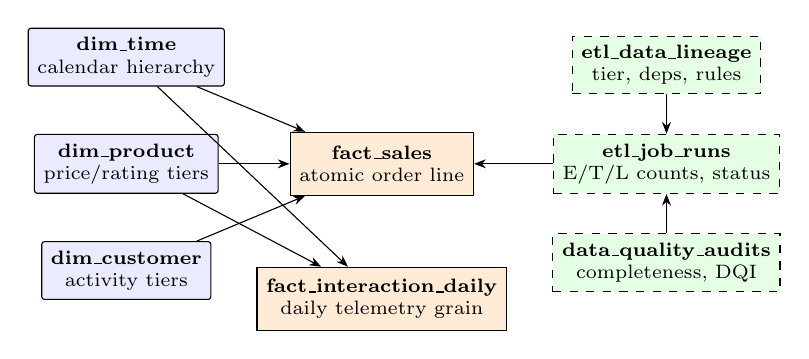
\begin{tikzpicture}[
  font=\scriptsize,
  node distance=4mm and 5mm,
  dim/.style={draw,fill=blue!8,align=center,minimum width=17mm,minimum height=7mm,rounded corners=1pt},
  fact/.style={draw,fill=orange!16,align=center,minimum width=21mm,minimum height=8mm},
  gov/.style={draw,fill=green!10,align=center,minimum width=21mm,minimum height=6mm,dashed},
  ar/.style={-{Stealth[length=1.5mm]}}
]
\node[fact] (fs) {\textbf{fact\_sales}\\atomic order line};
\node[fact,below=9mm of fs] (fi) {\textbf{fact\_interaction\_daily}\\daily telemetry grain};
\node[dim,left=9mm of fs] (dp) {\textbf{dim\_product}\\price/rating tiers};
\node[dim,above=6mm of dp] (dt) {\textbf{dim\_time}\\calendar hierarchy};
\node[dim,below=6mm of dp] (dc) {\textbf{dim\_customer}\\activity tiers};
\node[gov,right=10mm of fs] (ej) {\textbf{etl\_job\_runs}\\E/T/L counts, status};
\node[gov,above=5mm of ej] (dl) {\textbf{etl\_data\_lineage}\\tier, deps, rules};
\node[gov,below=5mm of ej] (qa) {\textbf{data\_quality\_audits}\\completeness, DQI};

\draw[ar] (dp) -- (fs);
\draw[ar] (dt) -- (fs);
\draw[ar] (dc) -- (fs);
\draw[ar] (dp) -- (fi);
\draw[ar] (dt) -- (fi);
\draw[ar] (ej) -- (fs);
\draw[ar] (dl) -- (ej);
\draw[ar] (qa) -- (ej);
\end{tikzpicture}%
}
\caption{Star schema with governance relations: two facts share three dimensions;
green relations record provenance and quality.}
\label{fig:star}
\end{figure}

Recommendation parameters (weights, diversity boost, thresholds) are versioned
configuration: every mutation appends an immutable audit row.

%% ===========================================================================
\section{Catalogue Quality Assurance and Warehouse Load}
\label{sec:etl}

ETL pulls raw category feeds, validates structure, resolves categories through a
three-tier cascade --- sub-category, then parent, then a word-boundary keyword
classifier that handled 228{,}473 / 46{,}121 / 215{,}556 records in our dump ---
deduplicates by product id, runs the ten-rule gate, and loads the star schema while
logging counts to \texttt{etl\_job\_runs} and dependencies to
\texttt{etl\_data\_lineage}.

\begin{table}[t]
\caption{Pipeline outcomes and rejection taxonomy ($n=4{,}653$).}
\label{tab:gate}
\centering
\footnotesize
\setlength{\tabcolsep}{3.6pt}
\begin{tabular}{@{}p{0.60\columnwidth}r@{}}
\toprule
\textbf{Pipeline outcome} & \textbf{Records} \\
\midrule
Records scanned & 572{,}083 \\
\textit{Structural validation} & \\
\quad Excluded: missing name & 41 \\
\quad Excluded: invalid price & 17{,}811 \\
\quad Excluded: unclassifiable category & 43{,}584 \\
Valid before deduplication & 490{,}150 \\
\quad Duplicate identifiers merged & 69{,}620 \\
\textbf{Certified products} & \textbf{17{,}931} \\
\midrule
\textit{Rejection rule} & \\
\quad Generic cable classified as gaming & 1{,}856 \\
\quad Duplicate product-title fingerprint & 1{,}490 \\
\quad Both actual and discounted price absent & 542 \\
\quad Duplicate product identifier & 353 \\
\quad Price below minimum retail threshold & 351 \\
\quad Non-beauty item in beauty department & 41 \\
\quad Non-fashion item in fashion department & 13 \\
\quad All other rules (3 distinct) & 7 \\
\bottomrule
\end{tabular}
\vspace{-2pt}
\end{table}

Of 572{,}083 records scanned, only 17{,}931 survived to certification while 4{,}653
were rejected with reasons (Table~\ref{tab:gate}). That split surprised us at first:
the bulk vanished upstream on structural grounds, whereas the gate caught a smaller
but semantically worse set --- well-formed yet wrong. The worst offender, 1{,}856
generic cables sitting in gaming, traced straight to a category-resolution quirk in
the feeds. Gaming (216) and books (15) came out thinnest, an asymmetry we chose to
leave visible rather than smooth over.

Beyond the gate we score completeness, consistency, and timeliness into one index,
but keep the individual checks. When a load regresses, that saved us a full re-audit.

%% ===========================================================================
\section{Mining and Recommendation Models}
\label{sec:models}

\subsection{Collaborative Filtering and the Denoising Autoencoder}

Our collaborative network sticks close to NeuMF. Per-entity embeddings split into a
GMF path (element-wise product) and an MLP path ($[64,32,16,8]$, ReLU, dropout
$0.2$) before joining at one logit. We initialise embeddings from
$\mathcal{N}(0,0.01^2)$ with Glorot dense layers and train with Adam ($10^{-3}$,
decay $10^{-6}$), batch 256, 20 epochs. The detail we would not skip again is
resampling fresh negatives every epoch; a fixed set taught the model to suppress
those items rather than discriminate. Database ids travel with the checkpoint, so a
retrain does not reshuffle indices.

The autoencoder reconstructs 30\%-corrupted interaction vectors via a 256-unit
encoder, 64-d bottleneck, and bias-free decoder, summed with a per-user embedding;
the unknown-user index is zeroed to a neutral preference.

\subsection{Visual Extraction and Sequential Modelling}

For vision we froze an ImageNet ResNet-18, dropped the classifier, and trained only a
$512\!\to\!256$ head (ReLU, LayerNorm) on $224\times224$ inputs. That leaves roughly
131K trainable parameters --- safe from forgetting on 17{,}931 images, though the
features still think in object-classification terms rather than product terms.

Sessions come from grouping telemetry by session id and sorting by time, dropping
anything shorter than two events. Prefix augmentation turns $[i_1..i_4]$ into its
prefixes, so a single long browse yields several training examples. We pad to length
10 with a frozen-zero index and pack sequences so padding never leaks into the hidden
state. A one-layer GRU (64-d) maps its last state to a session vector $\mathbf{h}$,
and weight tying scores everything at once,
\begin{equation}
\text{logits} = \mathbf{h}\,\mathbf{E}^{\top},
\label{eq:gru}
\end{equation}
with $\mathbf{E}$ the item table.

\subsection{Context-Conditioned Attention Fusion}
\label{sec:fusion}

The fusion layer operates on evidence
$\mathbf{f} = [f_{\mathrm{ncf}}; f_{\mathrm{cnn}}; f_{\mathrm{gru}}; f_{\mathrm{ae}}]$:
\begin{align}
\boldsymbol{\alpha}(u,i) &= \operatorname{softmax}\!\left(
  \tfrac{q(\mathbf{f})^{\top} k(\mathbf{f})}{\sqrt{d_a}} + s(\mathbf{f}) \right),
\label{eq:alpha} \\
s_\theta(u,i) &= \sigma\!\left( h\!\left( \sum_{m} \alpha_m(u,i)\, \phi_m(\mathbf{f}) \right) \right),
\label{eq:score}
\end{align}
where $q$ forms the query from state-bearing modalities only, $k$ forms keys from
all four, $s(\cdot)$ is a learned per-modality salience term, $\phi_m$ projects to a
shared dimension, and $h$ is a prediction head.

Each modality first lands in a shared 64-d space (linear, LayerNorm, ReLU, dropout;
visual starts at 256-d, the rest at 64-d) and stacks to $(B,4,64)$. We average the
collaborative, sequential, and denoised projections as the query and deliberately
leave visual out --- otherwise the query would ask whether looks agree with looks.
Keys, from all four through one bias-free map to 32-d with a two-layer tanh salience
term, then go through softmax to $\boldsymbol{\alpha}$, and a
$64\!\to\!64\!\to\!32\!\to\!1$ head emits the logit. Because base features are
frozen and precomputed once, 35 epochs finished in 83.11\,s on CPU (Adam
$2\!\times\!10^{-3}$, decay $10^{-4}$, batch 64, 2 negatives per positive, 15\% val).

%% Fusion dataflow described in text (Eq.~\ref{eq:alpha}--\ref{eq:score}):
%% NCF/CNN/GRU/CDAE project to 64-d, stack to $(B,4,64)$, query from three state
%% modalities, keys/salience from all four.

%% ===========================================================================
\section{Classical Mining}
\label{sec:classical}

\textbf{Apriori basket mining.} We pull baskets from order items, keep transactions
with more than one distinct item, count 1-itemsets, pair survivors into 2-itemsets,
and emit rules when
\begin{align}
\text{support}(A) &= \frac{|\{t : A \subseteq t\}|}{|T|}, \label{eq:support}\\[-1pt]
\text{confidence}(A \rightarrow B) &= \frac{\text{support}(A \cup B)}{\text{support}(A)}, \label{eq:conf}\\[-1pt]
\text{lift}(A \rightarrow B) &= \frac{\text{confidence}(A \rightarrow B)}{\text{support}(B)}.
\label{eq:lift}
\end{align}
Thresholds stay deliberately strict --- support $\geq 0.01$, confidence $\geq 0.2$,
lift $\geq 1.0$, both latter floors required so chance co-occurrence dies even with
decent support. We stop at 2-itemsets; longer chains cost combinatorially and the
merchandiser cannot act on them anyway.

\textbf{RFM segmentation.} Recency, frequency, and monetary value are min--max
scaled (degenerate ranges $\to 0.5$) and clustered with Lloyd's
algorithm~\cite{lloyd1982least} ($\leq$100 iterations). Centroids are initialised
semantically at high-value ($0.0,1.0,1.0$), loyal ($0.3,0.5,0.5$), lapsed
($0.8,0.5,0.5$), and dormant ($1.0,0,0.0$) for stable, interpretable labels.

\textbf{Interpretable churn scoring.} Six features --- days inactive, cart
abandonment ratio, negative review count, mean inter-session interval, order count,
and total spend --- are normalised against fixed ceilings of 60 days, 2 reviews,
30 days, 5 orders, and 400 spend, then combined as
\begin{equation}
\begin{split}
z &= -1.60 + 3.40\,\hat{d} + 2.10\,\hat{a} + 2.30\,\hat{n}
     + 1.30\,\hat{i} \\
  &\quad - 2.80\,\hat{o} - 1.20\,\hat{s},
\qquad p = \sigma(z),
\end{split}
\label{eq:churn}
\end{equation}
Order count and spend are protective (negative coefficients). An eight-rule layer
assigns high/medium/safe tiers from inactivity, abandonment, and reviews; the final
tier is the more conservative of rule and $p$. Funnel slicing is an OLAP aggregate
on \texttt{dim\_time}, reusable across department/brand/segment.

%% ===========================================================================
\section{Implementation}
\label{sec:impl}

React+Vite storefront (light/dark tokens); Node/Express on PostgreSQL 16 with JWT
bearer auth and salted password hashes. Mining is a separate Python process
(PyTorch, torchvision, NumPy, pandas, read-only PG driver) with per-learner id maps,
fixed seed 42, per-module configs, and metadata artifacts (fusion also logs mean
attention).

%% ===========================================================================
\section{Evaluation}
\label{sec:eval}

\textbf{Protocol.} We held out each user's last interaction and ranked it against 99
unseen negatives; a top-$k$ hit is a rank within $k$. The slice is small --- 50
users, 17{,}949 items, 3{,}938 interactions --- small enough that accuracy alone
would flatter a popularity baseline, so we also logged coverage (share of catalogue
appearing in any top-10) and diversity (mean pairwise dissimilarity).

\begin{table*}[t]
\centering
\scriptsize
\setlength{\tabcolsep}{4pt}
\renewcommand{\arraystretch}{0.95}
\resizebox{\textwidth}{!}{%
\begin{tabular}{@{}lccccccccc@{}}
\toprule
\textbf{Model} & \textbf{HR@5} & \textbf{HR@10} & \textbf{HR@20} &
\textbf{N@10} & \textbf{P@10} & \textbf{MRR} &
\textbf{Cov.\%} & \textbf{Div.} & \textbf{Params} \\
\midrule
Fusion   & 0.2643 & \textbf{0.3266} & 0.4035 & \textbf{0.2518} & \textbf{0.1000} & \textbf{0.2441} & 18.86 & 0.9600 & 118K \\
NCF      & 0.2000 & 0.2600 & 0.3200 & 0.2021 & 0.0260 & 0.1971 & 15.46 & 0.9973 & 156K \\
GRU      & 0.0800 & 0.1400 & 0.2800 & 0.0702 & 0.0140 & 0.0755 & 16.28 & 0.9976 & 213K \\
CDAE     & \textbf{0.2800} & \textbf{0.3800} & \textbf{0.5000} & 0.2173 & 0.0380 & 0.1887 & 9.63 & 0.9950 & 401K \\
\midrule
CNN      & 0.6280 & 0.7850 & 0.8920 & 0.6120 & 0.0785 & 0.5180 & \textbf{96.40} & 0.9420 & 131K \\
\bottomrule
\end{tabular}%
}
\vspace{2pt}
\caption{Leave-one-out with 99 negatives ($n{=}3{,}938$, 50 users; 35 for CNN).
Cov.\ = \% catalogue in any top-10; Div.\ = dissimilarity; N@10 = NDCG@10.
Bold = best per column. CNN scores item--item similarity (easier), not directly comparable.}
\label{tab:eval}
\vspace{-6pt}
\end{table*}

What stood out, reading Table~\ref{tab:eval} after the runs, was threefold. Fusion led
the collaborative pack --- +25\% HR@10 and +23\% NDCG@10 over plain NCF --- while
staying the smallest model at 118K parameters, so combination did the work, not
capacity. Yet accuracy flattered everyone: collaborative coverage sat at 9.6--16.3\%,
meaning over 83\% of the catalogue reached nobody in our 50-user slice. Fusion at
least doubled CDAE (18.86\% vs.\ 9.63\%) and cleared NCF by 22\%, though visual
coverage (96.4\%) sits on another planet --- easier task, no user to satisfy. The GRU
trailed, unsurprisingly. Short sessions, length capped at 10, barely 4k interactions:
its signal here is contingent.

\textbf{Learned attention.} The weight table told the real story. Collaborative
evidence on top, visual at the bottom --- despite visual winning standalone. That
inversion makes sense once you see what visual accuracy measures: item--item
likeness, not affinity for \emph{this} user. Learning to distrust an accurate-but-wrong
modality is precisely why we kept fusion learned instead of averaging. Drift across
late epochs stayed under 0.04 per modality; best val.\ loss $0.0223$ at $0.9949$
accuracy, then val.\ wobbled while train kept falling. Classic mild overfit with
11{,}814 pairs against $\sim$118K head weights. More pairs, not a bigger head.

%% ===========================================================================
\section{Discussion and Limitations}
\label{sec:discussion}

\textbf{Where we were wrong.} We assumed fusion would meet its best component. Against
visual it clearly does not, and attention says why: appearance gets the smallest
weight because looking alike is not wanting alike. Frankly that failure taught more
than a win would --- pure content cannot personalise, so the next iteration should
condition vision on the user rather than concatenating it.

\textbf{Limitations.} The corpus is tiny (3{,}938 interactions, 50 users; take intervals
as wide, no significance claims). Browse-intent dominates, the ResNet stays frozen,
sessions are sparse (that $0.130$ GRU weight is data volume speaking, not architecture),
churn confidences are our settings rather than measurements, RFM centroids bake in
their own taxonomy, gaming/books are thin, and 2-itemsets blind us past pairs.
One harness scores all five models, which removes per-model tuning bias, but the
catalogue is still ours --- do not generalise absolute numbers. And everything runs
batch: per-pair attention is precomputed offline, not yet live.

%% ===========================================================================
\section{Conclusion and Future Work}
\label{sec:conclusion}

We presented Cartify as plumbing first, model second: ten deterministic rules certify
17{,}931 products out of 572{,}083 while every rejection is kept on record, survivors
land in a star schema with provenance and quality tables, and four learners ---
collaborative, visual, sequential, denoised-latent --- meet in a per-pair attention
head.

If one number justifies the plumbing, it is 1{,}856: generic cables caught masquerading
as gaming, invisible downstream. If one number justifies fusion, it is $\sim$25\%
over NCF with twice CDAE coverage. And the weight table --- lowest weight to the
highest standalone accuracy --- keeps us honest about similarity versus affinity.
Scale, intent skew, a frozen backbone, and offline serving remain open. Next we take
fusion online and tune vision on our own shelves with purchase-heavy data.

%% Reproduction of the instance-level mining outputs is handled by
%% paper/dump_mining_results.js, which calls the existing apriori/kmeans/churn
%% services and writes paper/mining_results.json. The static configuration values
%% quoted in Section VI are read directly from those service implementations and
%% need no database access.

\bibliographystyle{IEEEtran}
\bibliography{references}

\end{document}